%%%%%%%%%%%%%%%%%%%%%%%%%%%%%%%%%%%%%%%%%%%%%%%%%%%%%%%%%%%%%%%%%%%%%%%%%%%%%%%%%%%%%%%%%%%%%%%%%%%%%%%%%%%%%%%%%%%%%%%%%%%%%%%%%%%%%%%%%%%%%%%%%%%%%%%%%%%%%%%%%%%
% Written By Michael Brodskiy
% Class: Electricity & Magnetism
% Professor: D. Wood
%%%%%%%%%%%%%%%%%%%%%%%%%%%%%%%%%%%%%%%%%%%%%%%%%%%%%%%%%%%%%%%%%%%%%%%%%%%%%%%%%%%%%%%%%%%%%%%%%%%%%%%%%%%%%%%%%%%%%%%%%%%%%%%%%%%%%%%%%%%%%%%%%%%%%%%%%%%%%%%%%%%

\documentclass[12pt]{article} 
\usepackage{alphalph}
\usepackage[utf8]{inputenc}
\usepackage[russian,english]{babel}
\usepackage{titling}
\usepackage{amsmath}
\usepackage{graphicx}
\usepackage{enumitem}
\usepackage{amssymb}
\usepackage[super]{nth}
\usepackage{everysel}
\usepackage{ragged2e}
\usepackage{geometry}
\usepackage{multicol}
\usepackage{fancyhdr}
\usepackage{cancel}
\usepackage{siunitx}
\usepackage{physics}
\usepackage{tikz}
\usepackage{mathdots}
\usepackage{yhmath}
\usepackage{cancel}
\usepackage{color}
\usepackage{array}
\usepackage{multirow}
\usepackage{gensymb}
\usepackage{tabularx}
\usepackage{extarrows}
\usepackage{booktabs}
\usepackage{lastpage}
\usetikzlibrary{fadings}
\usetikzlibrary{patterns}
\usetikzlibrary{shadows.blur}
\usetikzlibrary{shapes}

\geometry{top=1.0in,bottom=1.0in,left=1.0in,right=1.0in}
\newcommand{\subtitle}[1]{%
  \posttitle{%
    \par\end{center}
    \begin{center}\large#1\end{center}
    \vskip0.5em}%

}
\usepackage{hyperref}
\hypersetup{
colorlinks=true,
linkcolor=blue,
filecolor=magenta,      
urlcolor=blue,
citecolor=blue,
}


\title{Homework 2}
\date{September 28, 2023}
\author{Michael Brodskiy\\ \small Professor: D. Wood}

\begin{document}

\maketitle

\begin{enumerate}

  \item Six charges are arranged along the sides and corners of a square with sides of length L as shown. Calculate the magnitude and direction of the electric field at the origin. Use symmetry and superposition to make the calculation simple.

    \begin{center}
      \begin{figure}[H]
        \centering
        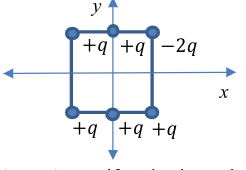
\includegraphics[width=.3\textwidth]{Figures/Figure2-1.png}
        \label{fig:1}
      \end{figure}
    \end{center}

    We know, by definition, that $\vec{F}=\vec{E}q$. Using the concepts we know about force, we know the following charges cancel out each other, as they are symmetric about the test charge at the origin:

    \begin{figure}[H]
      \centering
      \tikzset{every picture/.style={line width=0.75pt}} %set default line width to 0.75pt        

\begin{tikzpicture}[x=0.75pt,y=0.75pt,yscale=-1,xscale=1]
%uncomment if require: \path (0,430); %set diagram left start at 0, and has height of 430

%Shape: Grid [id:dp9511403020531122] 
\draw  [draw opacity=0] (225,103) -- (386,103) -- (386,264) -- (225,264) -- cycle ; \draw   (225,103) -- (225,264)(305,103) -- (305,264)(385,103) -- (385,264) ; \draw   (225,103) -- (386,103)(225,183) -- (386,183)(225,263) -- (386,263) ; \draw    ;
%Shape: Circle [id:dp026055485587581195] 
\draw  [color={rgb, 255:red, 74; green, 83; blue, 226 }  ,draw opacity=1 ][fill={rgb, 255:red, 74; green, 144; blue, 226 }  ,fill opacity=1 ][line width=1.5]  (219.5,103) .. controls (219.5,99.96) and (221.96,97.5) .. (225,97.5) .. controls (228.04,97.5) and (230.5,99.96) .. (230.5,103) .. controls (230.5,106.04) and (228.04,108.5) .. (225,108.5) .. controls (221.96,108.5) and (219.5,106.04) .. (219.5,103) -- cycle ;
%Shape: Circle [id:dp8849353673163125] 
\draw  [color={rgb, 255:red, 74; green, 83; blue, 226 }  ,draw opacity=1 ][fill={rgb, 255:red, 74; green, 144; blue, 226 }  ,fill opacity=1 ][line width=1.5]  (299.5,103) .. controls (299.5,99.96) and (301.96,97.5) .. (305,97.5) .. controls (308.04,97.5) and (310.5,99.96) .. (310.5,103) .. controls (310.5,106.04) and (308.04,108.5) .. (305,108.5) .. controls (301.96,108.5) and (299.5,106.04) .. (299.5,103) -- cycle ;
%Shape: Circle [id:dp7298663131993588] 
\draw  [color={rgb, 255:red, 74; green, 83; blue, 226 }  ,draw opacity=1 ][fill={rgb, 255:red, 74; green, 144; blue, 226 }  ,fill opacity=1 ][line width=1.5]  (379.5,103) .. controls (379.5,99.96) and (381.96,97.5) .. (385,97.5) .. controls (388.04,97.5) and (390.5,99.96) .. (390.5,103) .. controls (390.5,106.04) and (388.04,108.5) .. (385,108.5) .. controls (381.96,108.5) and (379.5,106.04) .. (379.5,103) -- cycle ;
%Shape: Circle [id:dp5118102160520555] 
\draw  [color={rgb, 255:red, 74; green, 83; blue, 226 }  ,draw opacity=1 ][fill={rgb, 255:red, 74; green, 144; blue, 226 }  ,fill opacity=1 ][line width=1.5]  (219.5,263) .. controls (219.5,259.96) and (221.96,257.5) .. (225,257.5) .. controls (228.04,257.5) and (230.5,259.96) .. (230.5,263) .. controls (230.5,266.04) and (228.04,268.5) .. (225,268.5) .. controls (221.96,268.5) and (219.5,266.04) .. (219.5,263) -- cycle ;
%Shape: Circle [id:dp9003932477737502] 
\draw  [color={rgb, 255:red, 74; green, 83; blue, 226 }  ,draw opacity=1 ][fill={rgb, 255:red, 74; green, 144; blue, 226 }  ,fill opacity=1 ][line width=1.5]  (299.5,263) .. controls (299.5,259.96) and (301.96,257.5) .. (305,257.5) .. controls (308.04,257.5) and (310.5,259.96) .. (310.5,263) .. controls (310.5,266.04) and (308.04,268.5) .. (305,268.5) .. controls (301.96,268.5) and (299.5,266.04) .. (299.5,263) -- cycle ;
%Shape: Circle [id:dp7160989607764205] 
\draw  [color={rgb, 255:red, 74; green, 83; blue, 226 }  ,draw opacity=1 ][fill={rgb, 255:red, 74; green, 144; blue, 226 }  ,fill opacity=1 ][line width=1.5]  (379.5,263) .. controls (379.5,259.96) and (381.96,257.5) .. (385,257.5) .. controls (388.04,257.5) and (390.5,259.96) .. (390.5,263) .. controls (390.5,266.04) and (388.04,268.5) .. (385,268.5) .. controls (381.96,268.5) and (379.5,266.04) .. (379.5,263) -- cycle ;
%Shape: Circle [id:dp693930431751913] 
\draw  [color={rgb, 255:red, 207; green, 248; blue, 28 }  ,draw opacity=1 ][fill={rgb, 255:red, 248; green, 231; blue, 28 }  ,fill opacity=1 ][line width=1.5]  (299.5,183) .. controls (299.5,179.96) and (301.96,177.5) .. (305,177.5) .. controls (308.04,177.5) and (310.5,179.96) .. (310.5,183) .. controls (310.5,186.04) and (308.04,188.5) .. (305,188.5) .. controls (301.96,188.5) and (299.5,186.04) .. (299.5,183) -- cycle ;
%Shape: Ellipse [id:dp5545063148136824] 
\draw  [color={rgb, 255:red, 208; green, 2; blue, 27 }  ,draw opacity=1 ] (305,68.5) .. controls (316.05,68.5) and (325,121.67) .. (325,187.25) .. controls (325,252.83) and (316.05,306) .. (305,306) .. controls (293.95,306) and (285,252.83) .. (285,187.25) .. controls (285,121.67) and (293.95,68.5) .. (305,68.5) -- cycle ;

% Text Node
\draw (217.5,103) node [anchor=east] [inner sep=0.75pt]    {$+q$};
% Text Node
\draw (217.5,263) node [anchor=east] [inner sep=0.75pt]    {$+q$};
% Text Node
\draw (305,94.1) node [anchor=south] [inner sep=0.75pt]    {$+q$};
% Text Node
\draw (305,271.9) node [anchor=north] [inner sep=0.75pt]    {$+q$};
% Text Node
\draw (392.5,263) node [anchor=west] [inner sep=0.75pt]    {$+q$};
% Text Node
\draw (392.5,103) node [anchor=west] [inner sep=0.75pt]    {$-2q$};


\end{tikzpicture}

      \caption{The Opposite Forces Negate Each Other}
      \label{fig:3}
    \end{figure}

    \begin{figure}[H]
      \centering
      \tikzset{every picture/.style={line width=0.75pt}} %set default line width to 0.75pt        

\begin{tikzpicture}[x=0.75pt,y=0.75pt,yscale=-1,xscale=1]
%uncomment if require: \path (0,430); %set diagram left start at 0, and has height of 430

%Shape: Grid [id:dp9511403020531122] 
\draw  [draw opacity=0] (225,103) -- (386,103) -- (386,264) -- (225,264) -- cycle ; \draw   (225,103) -- (225,264)(305,103) -- (305,264)(385,103) -- (385,264) ; \draw   (225,103) -- (386,103)(225,183) -- (386,183)(225,263) -- (386,263) ; \draw    ;
%Shape: Circle [id:dp026055485587581195] 
\draw  [color={rgb, 255:red, 74; green, 83; blue, 226 }  ,draw opacity=1 ][fill={rgb, 255:red, 74; green, 144; blue, 226 }  ,fill opacity=1 ][line width=1.5]  (219.5,103) .. controls (219.5,99.96) and (221.96,97.5) .. (225,97.5) .. controls (228.04,97.5) and (230.5,99.96) .. (230.5,103) .. controls (230.5,106.04) and (228.04,108.5) .. (225,108.5) .. controls (221.96,108.5) and (219.5,106.04) .. (219.5,103) -- cycle ;
%Shape: Circle [id:dp8849353673163125] 
\draw  [color={rgb, 255:red, 74; green, 83; blue, 226 }  ,draw opacity=1 ][fill={rgb, 255:red, 74; green, 144; blue, 226 }  ,fill opacity=1 ][line width=1.5]  (299.5,103) .. controls (299.5,99.96) and (301.96,97.5) .. (305,97.5) .. controls (308.04,97.5) and (310.5,99.96) .. (310.5,103) .. controls (310.5,106.04) and (308.04,108.5) .. (305,108.5) .. controls (301.96,108.5) and (299.5,106.04) .. (299.5,103) -- cycle ;
%Shape: Circle [id:dp7298663131993588] 
\draw  [color={rgb, 255:red, 74; green, 83; blue, 226 }  ,draw opacity=1 ][fill={rgb, 255:red, 74; green, 144; blue, 226 }  ,fill opacity=1 ][line width=1.5]  (379.5,103) .. controls (379.5,99.96) and (381.96,97.5) .. (385,97.5) .. controls (388.04,97.5) and (390.5,99.96) .. (390.5,103) .. controls (390.5,106.04) and (388.04,108.5) .. (385,108.5) .. controls (381.96,108.5) and (379.5,106.04) .. (379.5,103) -- cycle ;
%Shape: Circle [id:dp5118102160520555] 
\draw  [color={rgb, 255:red, 74; green, 83; blue, 226 }  ,draw opacity=1 ][fill={rgb, 255:red, 74; green, 144; blue, 226 }  ,fill opacity=1 ][line width=1.5]  (219.5,263) .. controls (219.5,259.96) and (221.96,257.5) .. (225,257.5) .. controls (228.04,257.5) and (230.5,259.96) .. (230.5,263) .. controls (230.5,266.04) and (228.04,268.5) .. (225,268.5) .. controls (221.96,268.5) and (219.5,266.04) .. (219.5,263) -- cycle ;
%Shape: Circle [id:dp9003932477737502] 
\draw  [color={rgb, 255:red, 74; green, 83; blue, 226 }  ,draw opacity=1 ][fill={rgb, 255:red, 74; green, 144; blue, 226 }  ,fill opacity=1 ][line width=1.5]  (299.5,263) .. controls (299.5,259.96) and (301.96,257.5) .. (305,257.5) .. controls (308.04,257.5) and (310.5,259.96) .. (310.5,263) .. controls (310.5,266.04) and (308.04,268.5) .. (305,268.5) .. controls (301.96,268.5) and (299.5,266.04) .. (299.5,263) -- cycle ;
%Shape: Circle [id:dp7160989607764205] 
\draw  [color={rgb, 255:red, 74; green, 83; blue, 226 }  ,draw opacity=1 ][fill={rgb, 255:red, 74; green, 144; blue, 226 }  ,fill opacity=1 ][line width=1.5]  (379.5,263) .. controls (379.5,259.96) and (381.96,257.5) .. (385,257.5) .. controls (388.04,257.5) and (390.5,259.96) .. (390.5,263) .. controls (390.5,266.04) and (388.04,268.5) .. (385,268.5) .. controls (381.96,268.5) and (379.5,266.04) .. (379.5,263) -- cycle ;
%Shape: Circle [id:dp693930431751913] 
\draw  [color={rgb, 255:red, 207; green, 248; blue, 28 }  ,draw opacity=1 ][fill={rgb, 255:red, 248; green, 231; blue, 28 }  ,fill opacity=1 ][line width=1.5]  (299.5,183) .. controls (299.5,179.96) and (301.96,177.5) .. (305,177.5) .. controls (308.04,177.5) and (310.5,179.96) .. (310.5,183) .. controls (310.5,186.04) and (308.04,188.5) .. (305,188.5) .. controls (301.96,188.5) and (299.5,186.04) .. (299.5,183) -- cycle ;
%Shape: Ellipse [id:dp5545063148136824] 
\draw  [color={rgb, 255:red, 208; green, 2; blue, 27 }  ,draw opacity=1 ] (197.25,75.25) .. controls (215.06,57.44) and (277.74,91.24) .. (337.25,150.75) .. controls (396.76,210.26) and (430.56,272.94) .. (412.75,290.75) .. controls (394.94,308.56) and (332.26,274.76) .. (272.75,215.25) .. controls (213.24,155.74) and (179.44,93.06) .. (197.25,75.25) -- cycle ;

% Text Node
\draw (217.5,103) node [anchor=east] [inner sep=0.75pt]    {$+q$};
% Text Node
\draw (217.5,263) node [anchor=east] [inner sep=0.75pt]    {$+q$};
% Text Node
\draw (305,94.1) node [anchor=south] [inner sep=0.75pt]    {$+q$};
% Text Node
\draw (305,271.9) node [anchor=north] [inner sep=0.75pt]    {$+q$};
% Text Node
\draw (392.5,263) node [anchor=west] [inner sep=0.75pt]    {$+q$};
% Text Node
\draw (392.5,103) node [anchor=west] [inner sep=0.75pt]    {$-2q$};


\end{tikzpicture}

      \caption{The Opposite Forces Negate Each Other}
      \label{fig:4}
    \end{figure}

    Thus, we need only consider the effects of these charges:

    \begin{figure}[H]
      \centering
      \tikzset{every picture/.style={line width=0.75pt}} %set default line width to 0.75pt        

\begin{tikzpicture}[x=0.75pt,y=0.75pt,yscale=-1,xscale=1]
%uncomment if require: \path (0,430); %set diagram left start at 0, and has height of 430

%Shape: Grid [id:dp9511403020531122] 
\draw  [draw opacity=0] (225,103) -- (386,103) -- (386,264) -- (225,264) -- cycle ; \draw   (225,103) -- (225,264)(305,103) -- (305,264)(385,103) -- (385,264) ; \draw   (225,103) -- (386,103)(225,183) -- (386,183)(225,263) -- (386,263) ; \draw    ;
%Shape: Circle [id:dp026055485587581195] 
\draw  [color={rgb, 255:red, 74; green, 83; blue, 226 }  ,draw opacity=1 ][fill={rgb, 255:red, 74; green, 144; blue, 226 }  ,fill opacity=1 ][line width=1.5]  (219.5,103) .. controls (219.5,99.96) and (221.96,97.5) .. (225,97.5) .. controls (228.04,97.5) and (230.5,99.96) .. (230.5,103) .. controls (230.5,106.04) and (228.04,108.5) .. (225,108.5) .. controls (221.96,108.5) and (219.5,106.04) .. (219.5,103) -- cycle ;
%Shape: Circle [id:dp8849353673163125] 
\draw  [color={rgb, 255:red, 74; green, 83; blue, 226 }  ,draw opacity=1 ][fill={rgb, 255:red, 74; green, 144; blue, 226 }  ,fill opacity=1 ][line width=1.5]  (299.5,103) .. controls (299.5,99.96) and (301.96,97.5) .. (305,97.5) .. controls (308.04,97.5) and (310.5,99.96) .. (310.5,103) .. controls (310.5,106.04) and (308.04,108.5) .. (305,108.5) .. controls (301.96,108.5) and (299.5,106.04) .. (299.5,103) -- cycle ;
%Shape: Circle [id:dp7298663131993588] 
\draw  [color={rgb, 255:red, 74; green, 83; blue, 226 }  ,draw opacity=1 ][fill={rgb, 255:red, 74; green, 144; blue, 226 }  ,fill opacity=1 ][line width=1.5]  (379.5,103) .. controls (379.5,99.96) and (381.96,97.5) .. (385,97.5) .. controls (388.04,97.5) and (390.5,99.96) .. (390.5,103) .. controls (390.5,106.04) and (388.04,108.5) .. (385,108.5) .. controls (381.96,108.5) and (379.5,106.04) .. (379.5,103) -- cycle ;
%Shape: Circle [id:dp5118102160520555] 
\draw  [color={rgb, 255:red, 74; green, 83; blue, 226 }  ,draw opacity=1 ][fill={rgb, 255:red, 74; green, 144; blue, 226 }  ,fill opacity=1 ][line width=1.5]  (219.5,263) .. controls (219.5,259.96) and (221.96,257.5) .. (225,257.5) .. controls (228.04,257.5) and (230.5,259.96) .. (230.5,263) .. controls (230.5,266.04) and (228.04,268.5) .. (225,268.5) .. controls (221.96,268.5) and (219.5,266.04) .. (219.5,263) -- cycle ;
%Shape: Circle [id:dp9003932477737502] 
\draw  [color={rgb, 255:red, 74; green, 83; blue, 226 }  ,draw opacity=1 ][fill={rgb, 255:red, 74; green, 144; blue, 226 }  ,fill opacity=1 ][line width=1.5]  (299.5,263) .. controls (299.5,259.96) and (301.96,257.5) .. (305,257.5) .. controls (308.04,257.5) and (310.5,259.96) .. (310.5,263) .. controls (310.5,266.04) and (308.04,268.5) .. (305,268.5) .. controls (301.96,268.5) and (299.5,266.04) .. (299.5,263) -- cycle ;
%Shape: Circle [id:dp7160989607764205] 
\draw  [color={rgb, 255:red, 74; green, 83; blue, 226 }  ,draw opacity=1 ][fill={rgb, 255:red, 74; green, 144; blue, 226 }  ,fill opacity=1 ][line width=1.5]  (379.5,263) .. controls (379.5,259.96) and (381.96,257.5) .. (385,257.5) .. controls (388.04,257.5) and (390.5,259.96) .. (390.5,263) .. controls (390.5,266.04) and (388.04,268.5) .. (385,268.5) .. controls (381.96,268.5) and (379.5,266.04) .. (379.5,263) -- cycle ;
%Shape: Circle [id:dp693930431751913] 
\draw  [color={rgb, 255:red, 207; green, 248; blue, 28 }  ,draw opacity=1 ][fill={rgb, 255:red, 248; green, 231; blue, 28 }  ,fill opacity=1 ][line width=1.5]  (299.5,183) .. controls (299.5,179.96) and (301.96,177.5) .. (305,177.5) .. controls (308.04,177.5) and (310.5,179.96) .. (310.5,183) .. controls (310.5,186.04) and (308.04,188.5) .. (305,188.5) .. controls (301.96,188.5) and (299.5,186.04) .. (299.5,183) -- cycle ;
%Shape: Ellipse [id:dp5545063148136824] 
\draw  [color={rgb, 255:red, 126; green, 211; blue, 33 }  ,draw opacity=1 ] (421.88,73.88) .. controls (441.83,93.83) and (408.58,159.42) .. (347.63,220.38) .. controls (286.67,281.33) and (221.08,314.58) .. (201.13,294.63) .. controls (181.17,274.67) and (214.42,209.08) .. (275.38,148.13) .. controls (336.33,87.17) and (401.92,53.92) .. (421.88,73.88) -- cycle ;

% Text Node
\draw (217.5,103) node [anchor=east] [inner sep=0.75pt]    {$+q$};
% Text Node
\draw (217.5,263) node [anchor=east] [inner sep=0.75pt]    {$+q$};
% Text Node
\draw (305,94.1) node [anchor=south] [inner sep=0.75pt]    {$+q$};
% Text Node
\draw (305,271.9) node [anchor=north] [inner sep=0.75pt]    {$+q$};
% Text Node
\draw (392.5,263) node [anchor=west] [inner sep=0.75pt]    {$+q$};
% Text Node
\draw (392.5,103) node [anchor=west] [inner sep=0.75pt]    {$-2q$};


\end{tikzpicture}

      \caption{These Charges Remain Relevant}
      \label{fig:5}
    \end{figure}

    Using superposition, we know that the two charges can be summed, and they produce a horizontal force proportional to $3q$ at an angle of $\frac{\pi}{4}$ radians with respect to the $x$-axis. Decomposing this, we know the force can be expressed, with $Q$ as the test charge, as:

    $$E_Q=\frac{(3q)}{4\pi\varepsilon_o R^2}\cos\left( \frac{\pi}{4} \right)\bold{\hat{x}}+\frac{(3q)}{4\pi\varepsilon_o R^2}\sin\left( \frac{\pi}{4} \right)\bold{\hat{y}}$$

    Additionally, we know that $R=\sqrt{\left( \frac{L}{2} \right)^2+\left( \frac{L}{2} \right)^2}=\sqrt{\frac{L^2}{2}}=\frac{L}{\sqrt{2}}$. This gives us:

    $$\boxed{E_Q=\frac{3\sqrt{2}q}{4\pi\varepsilon_o L^2}\bold{\hat{x}}+\frac{3\sqrt{2}q}{4\pi\varepsilon_o L^2}\bold{\hat{y}}}$$

    It can also be said that the field, in the direction of the $-2q$ charge, is:

    $$\boxed{E_Q=\frac{3q}{2\pi\varepsilon_o L^2}\bold{\hat{-2q}}}$$

  \item A uniformly charged rod of length $L$ and charge $q$ is placed along the $x$-axis with its center at $x=a$. Find the $x$-component of the electric field at a point on the $z$ axis. (Hint: use $R$ as the variable of integration.) Check your expression in the following limit: $z=0$ and $a>>L$.

    \begin{center}
      \begin{figure}[H]
        \centering
        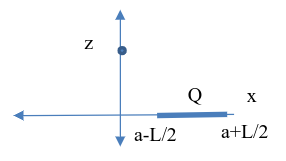
\includegraphics[width=.4\textwidth]{Figures/Figure2-2.png}
        \label{fig:2}
      \end{figure}
    \end{center}

    We know the rod is length $L$, with charge $Q$. This means the linear charge density can be defined as:

    $$\lambda=\frac{Q}{L}$$

    Furthermore, we can refer to the angle between the test charge and point on the rod as $\theta$, measured in the counter-clockwise direction, and the distance from said point on the rod to the test charge can be called $R$. This yields us the following expression for the $x$-axis:

    $$E_x=-\int \frac{\sin(\theta)}{4\pi\varepsilon_oR^2}\,dQ$$

    We can express $dq\rightarrow \lambda\,dx$, which gives us:

    $$E_x=-\int \frac{\lambda\sin(\theta)}{4\pi\varepsilon_oR^2}\,dx$$

    Then, if we were to assume $x$ as the horizontal distance from the test charge to the rod, and $z$ as the vertical distance from the test charge to the rod, we may see that: 

    $$\tan(\theta)=\frac{x}{z}$$
    $$z\tan(\theta)=x$$
    $$z\sec^2(\theta)\,d\theta=dx$$

    Taking $R$ into account, we can further simplify our calculation:

    $$\frac{dx}{R^2}=\frac{z\,d\theta}{R^2\cos^2(\theta)}$$

    Again referring to our set up, we know $\cos(\theta)=\dfrac{z}{R}$:

    $$dx=\frac{d\theta}{z}$$

    Finally, we can use this:

    $$E_x=-\frac{\lambda}{4\pi\varepsilon_o z}\int_{\theta_{a-\frac{L}{2}}}^{\theta_{a+\frac{L}{2}}} \sin(\theta)\,d\theta$$
    $$\frac{\lambda}{4\pi\varepsilon_o z}\left[ \cos(\theta) \right]\Big|_{\theta_{a-\frac{L}{2}}}^{\theta_{a+\frac{L}{2}}}$$

    We can once again refer to the set-up, finding that:

    $$\left\{\begin{array}{l c c}\cos(\theta_{a-\frac{L}{2}})=\frac{z}{\sqrt{z^2+(a-L/2)^2}}\\\cos(\theta_{a+\frac{L}{2}})=\frac{z}{\sqrt{z^2+(a+L/2)^2}}\\\end{array}$$

      Substituting this into our final expression, we get:

      $$\boxed{\frac{\lambda}{4\pi\varepsilon_o}\left( \frac{1}{\sqrt{z^2+(a+L/2)^2}}-\frac{1}{\sqrt{z^2+(a-L/2)^2}} \right)}$$

      \textsc{$z=0$ case:}

      $$\frac{\lambda}{4\pi\varepsilon_o}\left( \frac{1}{a+L/2}-\frac{1}{a-L/2} \right)$$
      $$\frac{\lambda}{4\pi\varepsilon_o}\left( \frac{a-L/2-(a+L/2)}{a^2-(L/2)^2} \right)$$
      $$-\frac{\lambda L}{(4\pi\varepsilon_o)(a^2-(L/2)^2)}$$
      $$-\frac{Q}{(4\pi\varepsilon_o)(a^2-(L/2)^2)}$$

      \textsc{$a>>L$ case:}

      $$\frac{\lambda}{4\pi\varepsilon_o}\left( \frac{1}{\sqrt{z^2+(a+L/2)^2}}-\frac{1}{\sqrt{z^2+(a-L/2)^2}} \right);\quad a\pm L\to 0$$
      $$\frac{\lambda}{4\pi\varepsilon_o}\cancel{\left( \frac{1}{\sqrt{z^2+a^2}}-\frac{1}{\sqrt{z^2+a^2}} \right)}=0$$

      This makes sense, as, logically, if the rod were centered at a point very far away from the test charge, there would be no significant electric field.
    
  \item Calculate the electric potential on the $z$-axis due to a uniformly charged annulus in the $xy$-plane centered at the origin with inner radius $a$ and outer radius $b$. Then find the electric field from the gradient of the potential.

    Let us assume the annulus holds a charge of $q$, with an area $A$. This defines the charge density as:

    $$\sigma=\frac{q}{A}$$

    This gives us:

    $$dq=\sigma dA$$

    If we assume that $i$ and $j$ are the horizontal and vertical distances, respectively, to the test charge from any point on the annulus, and $r=\sqrt{i^2+j^2}$ is the radial distance from the test charge to any point, then we can express the above as:

    $$dq=\sigma (2\pi i\,di)$$

    We can then define the voltage as:

    $$V=\frac{q}{4\pi\varepsilon_o r}$$
    $$dV=\frac{dq}{4\pi\varepsilon_o r}$$
    $$dV=\frac{\sigma i\,di}{2\varepsilon_o\sqrt{i^2+j^2}}$$

    We can then integrate to find the voltage expression:

    $$V=\frac{\sigma}{2\varepsilon_o}\int_a^b\frac{i}{\sqrt{i^2+j^2}}\,di$$

    Using $u$ substitution, with $u=i^2+j^2$, we get:

    $$V=\frac{\sigma}{\varepsilon_o}\int_{a^2+j^2}^{b^2+j^2}\frac{1}{\sqrt{u}}\,du$$
    $$V=\frac{\sigma}{\varepsilon_o}\left(  \frac{\sqrt{u}}{2}\right)\Big|_{a^2+j^2}^{b^2+j^2}$$
    $$V=\frac{\sigma}{2\varepsilon_o}\left(  \sqrt{j^2+b^2}-\sqrt{j^2+a^2}\right)$$

    We can then find the electric field using the gradient formula:

    $$\vec{E}=-\vec{\nabla}V$$
    $$\vec{E}=-\vec{\nabla}\left(  \frac{\sigma}{2\varepsilon_o}\left(  \sqrt{j^2+b^2}-\sqrt{j^2+a^2}\right) \right)$$
    $$\boxed{\vec{E}=\langle 0, 0, \frac{\sigma}{4\varepsilon_o}\left( \frac{j}{\sqrt{j^2+a^2}}-\frac{j}{\sqrt{j^2+b^2}} \right)\rangle}$$

    Because $j$ simply indicates the $z$ direction, and the vector above is with respect to the $i,j,k$ vectors, we can rewrite this as:

    $$\boxed{\vec{E}=\frac{\sigma}{4\varepsilon_o}\left( \frac{z}{\sqrt{z^2+a^2}}-\frac{z}{\sqrt{z^2+b^2}} \right)\bold{\hat{k}}}$$
    
  \item Consider an infinitely long uniformly-charged solid cylinder of radius $a$ and charge per unit volume $\rho$ surrounded by a coaxial cylindrical shell of radius $b$ and charge per unit area of $\sigma$. Take the axis of the cylinders as the $z$-axis.

    \begin{enumerate}

      \item Calculate the electric field everywhere in space

      \item Also calculate the potential as a function of the distance from the axis, taking the potential to be zero on the $z$-axis.

    \end{enumerate}
    
  \item The electric field for two charged concentric spherical shells is given by

    $$\left\{\begin{array}{c c} 0, & r<a\\ \bold{\hat{r}}A_1/r^2, & a< r< b\\ \bold{\hat{r}}A_2/r^2, & r>b \end{array}$$

      Where $A_1=5\times 10^6\left[ \frac{\si{\newton\meter\squared}}{\si{\coulomb}} \right]$, $A_2=-3\times10^6\left[ \frac{\si{\newton\meter\squared}}{\si{\coulomb}} \right]$, $a=.25[\si{\meter}]$, and $b=.45[\si{\meter}]$. Find the surface charge densities $\sigma_a$ and $\sigma_b$ on the two shells.
    
\end{enumerate}

\end{document}

